\chapter{Energy disaggregation assisted by appliance state sensing}\label{chap5}

In this chapter, we propose an energy disaggregation algorithm. It uses our appliance state sensing system to determine states of appliances, and uses a central energy meter to provide power numbers in Watts. 

\section{Energy disaggregation algorithm}

The sensors can tell when and which appliance power state has changed. However, it has no capability to provide power consumption numbers. With the knowledge of the aggregated power consumption, we are able to associate events with the changes in total consumption, so that we are able to infer the consumption of that particular appliance, assuming its consumption is stable when it is powered on. 

There are some challenges to do so. Firstly, there is usually slight variation in the power that an appliance takes over time. Some appliances have stable power traces, such as lights, others may have large variations in their power traces. We see 5W-10W variation in the power traces of laptops when simply browsing web pages. When there are a number of appliances, the variation adds up at the central meter, so that we usually see a very noisy power trace. Most of the appliances in our experiments consume tens of watts, and the variation is sometimes at the same order of magnitude. Therefore, even knowing there is an event happening, it is hard to tell the accurate power step change. We can not use a lowpass filter, because the high frequency noises are in the same frequency range as the step changes. 

Secondly, power changes observed at the central meter may not be synchronous with the events. The time difference can be as long as several seconds. In the case when multiple events happens close in time, the power trace goes as a slope, instead of having sharp steps. 

To overcome these problems, we run piecewise constant (PWC) denoising algorithm on the central power trace first. It estimates the original signal with a piecewise constant signal which only have a small number of step changes, removing the noise. The algorithm is discussed in the next section in detail. After PWC denoising, we match the step changes with the events, according to their timestamp. If an event is clear without overlapping with other events, we will have its associated power number. However, if multiple events happens close to each other, i.e they are overlapping, then further disaggregation is needed to get the power number for each individual event. The block diagram of the energy disaggregation algorithm is shown in Fig.\ref{fig:algooverview}. 

\begin{figure}[htb]
  \centering
  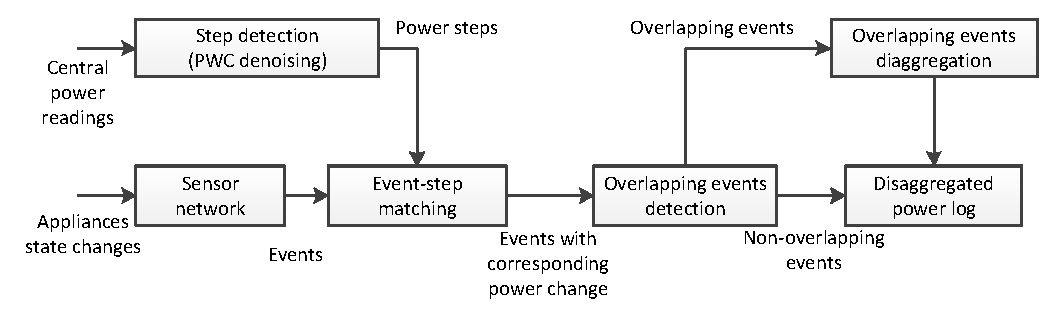
\includegraphics[width=\textwidth]{figures/algooverview}
  \caption{Block diagram of an energy disaggregation algorithm}
  \label{fig:algooverview}
\end{figure}

\subsection{PWC denoising and step detection with the central power trace}

In our experiments, we found that it is important to have a robust PWC denoising algorithm, especially when the number of appliances scales up and the interested appliances consume only tens or a hundred watts. Step changes in the aggregated power are swamped in noise.  A low pass filter is not suitable in this case because the noises have the same frequency as the step changes that we want to preserve. 
 The problem is not particularly significant in previous research, because previously, people mostly focus on few appliances with very large power consumption, such as dish washers, heaters or ovens.
 
Several methods have been used in previous work to remove noise or detect step-change in the power trace. In \cite{Hart1992}, the author developed an edge detection algorithm. It looks for stable periods where the variation is less than a threshold (15W or VAR). The method works only when the step changes are much larger than the variation, which is not true in our case. In \cite{Norford1996}, the authors used a median filter to remove spikes in the raw signal. Total variation denoising is used in \cite{Kolter2012}. The method can effectively remove noises in the signal and preserve steps. However, its purpose is not step detection. Hence, its output is not guaranteed to be a piecewise constant signal with sparse steps. 

A method called jump penalization is introduced in \cite{Little2011}. The original method is an offline one. The algorithm begins with a constant signal as the estimation of the input signal. Usually the mean or median value is used for the initial estimation. In each iteration, a greedy search tries to insert the best new step-change in the current estimation. The algorithm ends when the improvement of estimation accuracy by inserting new step-changes is too small. The algorithm guarantees piecewise constant output, and the step-changes are explicitly found in each iteration. 

In this work, we adopt the algorithm to an online variant, which can process the data in real time.  Instead of inserting step-changes iteratively, we insert step-changes one by one as new samples come in. When new samples come in, we consider adding at most one new step in the period of time from last step-change to the current sample. The flow chart of our step-detection algorithm is shown in Fig.\ref{fig:pwc}. The error function is defined as following: \[E(x,y) = \frac{1}{2} \sum_n \left(x_n - y_n\right)^2\]

\begin{figure}[htb]
  \centering
  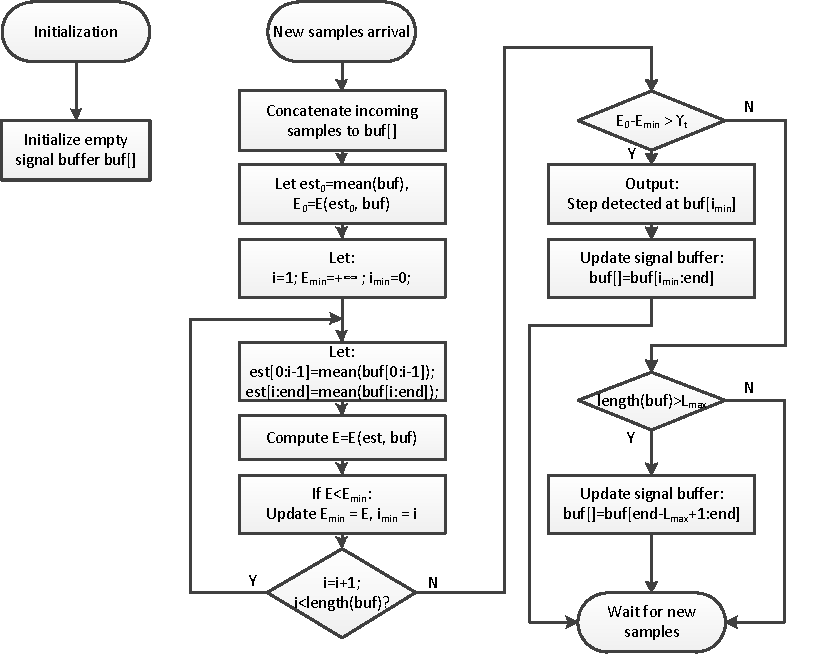
\includegraphics[width=\textwidth]{figures/pwc}
  \caption{Modified jump penalization algorithm for step detection}
  \label{fig:pwc}
\end{figure}

The parameter $\gamma$ acts as a threshold in the algorithm, or 'penalty' to insert a new step-change. With a lower $\gamma$, the output contains more steps. Instead of a constant $\gamma$, We use a time-variant $\gamma_t$ based on our knowledge about events. When there are events detected by the sensor network, we use the lower $\gamma_l$ so that it is more likely to detect small step changes. When no events are detected, we use the higher $\gamma_h$ to reduce false alarms. In practice, when the power signal is in kW, we choose $\gamma_l = 0.0001$ and $\gamma_h=0.0025$. 

We also limit the length of signal buffer to $L_{max}$, so that the greedy search domain is limited to the last $L_{max}$ samples. Otherwise, the buffer can grow indefinitely when there is no step-change for a long time. 

\subsection{Overlapping events disaggregation}

When multiple events happen close enough, only the aggregated effect will shown on the power readings at the central meter. In this case, we use the historical data to estimate the power changes. Specifically, we use the median value of all power changes that we observed before on non-overlapping events of a particular appliance. This works under the assumption that all appliances have binary on-off states.

\section{Experimental results}

We deployed an experimental setup in our lab. It is a mixed office and lab setting. All the interested appliances are arranged on 4 branch circuits, in order to minimize the interference from other appliances. The lab has 20 branch circuits in total, which is monitored by a Veris E30A panel energy meter\footnote{http://www.veris.com/}. We collect data from the meter at an interval of 2 seconds, and use the sum of power readings on the 4 branch circuits as the aggregated power reading.

We have 20 sensor nodes deployed, including 9 LCD monitors, 8 laptop computers, a solder station, a workbench light and a water dispenser. Most appliances are binary-state, except the water dispenser, which has both cooler and heater, and they work independently like two separate appliances. 

There are 11 appliances that we have instrumented with \textit{Watts up? PRO} meters. These meters capture the power consumption of individual appliances and log the data on a server through Gumstix nodes. These data serve as the ground truth. They are not used in any way in the energy disaggregation and inferencing process. 

The dataset used in this section is a 7-day long dataset collected from June 1st-7th, 2012. 

\subsection{Step detection results}

Fig.\ref{fig:pwc-example} shows some signal snippets with PWC denoising and step detection results. The big steps showing in the figure is the water dispenser heater. Except that, other power steps are mostly tens of Watts. And there is a oscillating noise in the power signal due to some laptop computers. The PWC denoising algorithm can detect steps in the same order of magnitude as the noise. 

\begin{figure}[htbp]
    \centering
    \begin{subfigure}[t]{0.47\textwidth}
        \centering
        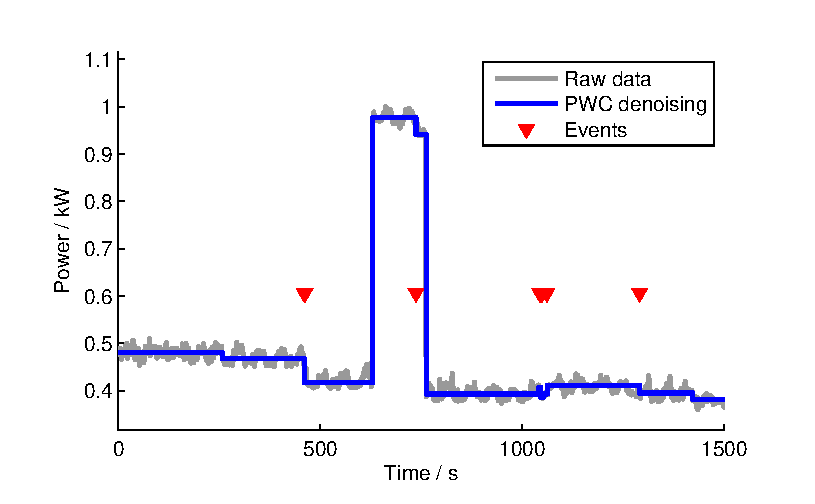
\includegraphics[width=\textwidth] {../../sw/pc/matlab/pwc-result/1.eps}
        \caption{}
    \end{subfigure} 
    \begin{subfigure}[t]{0.47\textwidth}
        \centering
        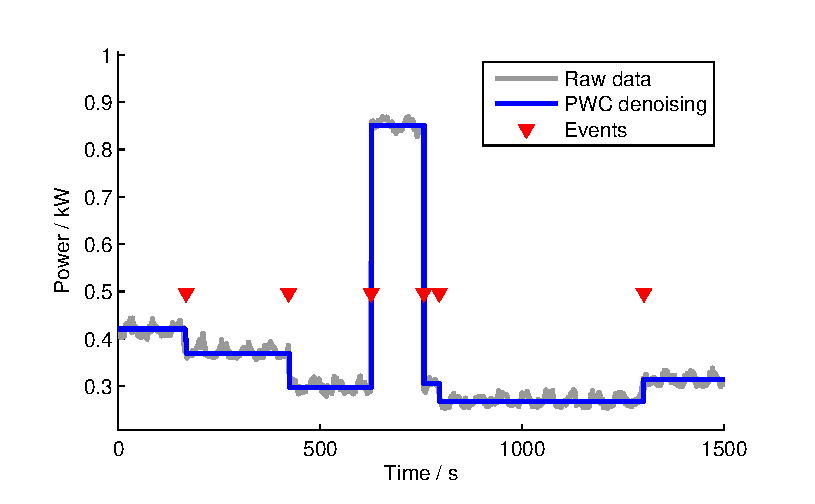
\includegraphics[width=\textwidth] {../../sw/pc/matlab/pwc-result/2.eps}
        \caption{}
    \end{subfigure} 
    \\
    \begin{subfigure}[t]{0.47\textwidth}
        \centering
        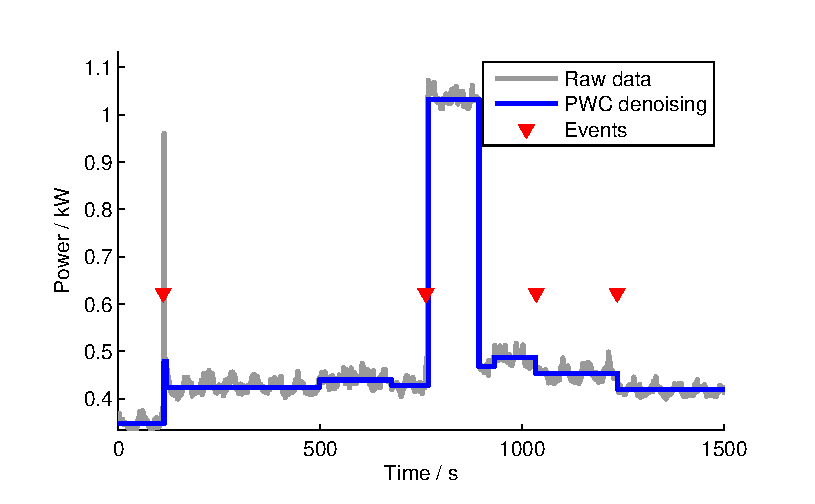
\includegraphics[width=\textwidth] {../../sw/pc/matlab/pwc-result/3.eps}
        \caption{}
    \end{subfigure} 
    \begin{subfigure}[t]{0.47\textwidth}
        \centering
        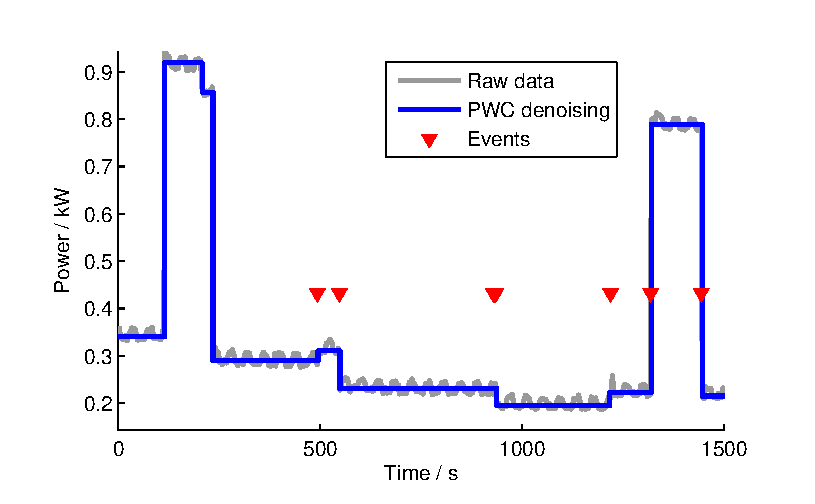
\includegraphics[width=\textwidth] {../../sw/pc/matlab/pwc-result/4.eps}
        \caption{}
    \end{subfigure} 
    \caption{Signal snippets showing PWC denoising results}\label{fig:pwc-example}
\end{figure}

\subsection{Appliance state tracking accuracy}

We use the state change events that the sensors detected to reconstruct the state of each individual appliances over time. By comparing appliance states collected by our sensors with the ground truth, we show the accuracy of our system. We measure accuracy by precision and recall, defined as following:
\[
\text{Precision} = \frac{tp}{tp+fp} = 
\frac{\text{Time appliance is on and reported on}}
{\text{Time appliance is reported on}}
\]
\[
\text{Recall} = \frac{tp}{tp+fn} = 
\frac{\text{Time appliance is on and reported on}}
{\text{Time appliance is on}}
\]

Table \ref{tab:pre-recall} shows the statistics of state tracking with ground truth. Here, an appliance is considered in on state when its power consumption is greater than 5W. The table shows power-on time, reported-on time, reported-on-and-indeed-on time, along with precision and recall. Fig.\ref{fig:state-1-2-3-5}-\ref{fig:state-17-18-21} shows the power consumption over time of the appliances. The solid traces are power ground truth of each individual appliance. Shaded area shows the period when our sensors report power-on. We can tell from the data that our system can provide very reliable and accurate appliance state data.

\begin{table}
  \centering
  \begin{tabular}{lccccc}
  \hline
  ID & On (s) & Reported on (s) & On\&reported on (s) & Precision (\%) & Recall (\%) \\
  \hline
1  & 24659  & 24586  & 24577   &99.965 &99.667 \\
2  & 24657  & 24586  & 24571   &99.937 &99.651 \\
3  & 19125  & 19131  & 19117   &99.925 &99.958 \\
5  & 136328 & 135248 & 135214  &99.975 &99.183 \\
8  & 19477  & 19477  & 19461   &99.920 &99.918 \\
12 & 128745 & 128198 & 128173  &99.981 &99.556 \\
13 & 106761 & 106200 & 106151  &99.954 &99.429 \\
14 & 764    & 763.7  & 762     &99.773 &99.738 \\
17 & 75308  & 75471  & 75296   &99.768 &99.984 \\
18 & 218431 & 217935 & 217771  &99.925 &99.698 \\
21 & 34720  & 34708  & 34642   &99.810 &99.775 \\
  \hline
  \end{tabular}
  \caption{Appliance state detection accuracy}
  \label{tab:pre-recall}
\end{table}


\begin{figure}[p]
    \centering
    \begin{subfigure}[t]{0.8\textwidth}
        \centering
        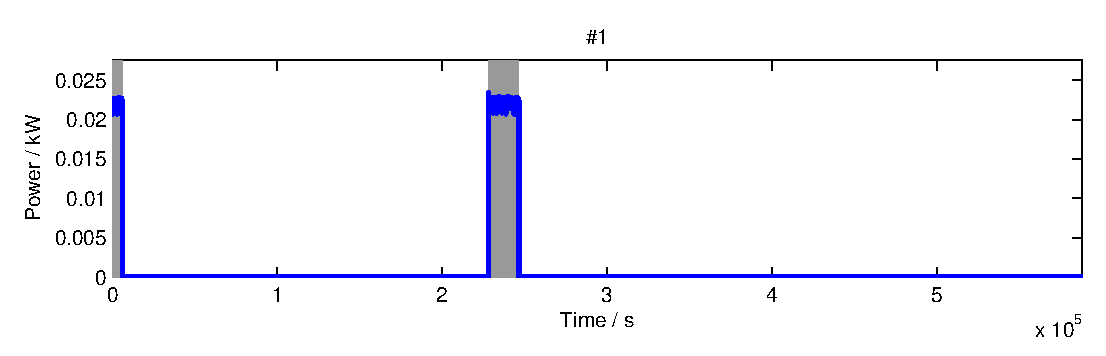
\includegraphics[width=\textwidth] {../../sw/pc/matlab/disagg-result/state-1.eps}
        \caption{\#1 Monitor}
    \end{subfigure} 
    \\
    \begin{subfigure}[t]{0.8\textwidth}
        \centering
        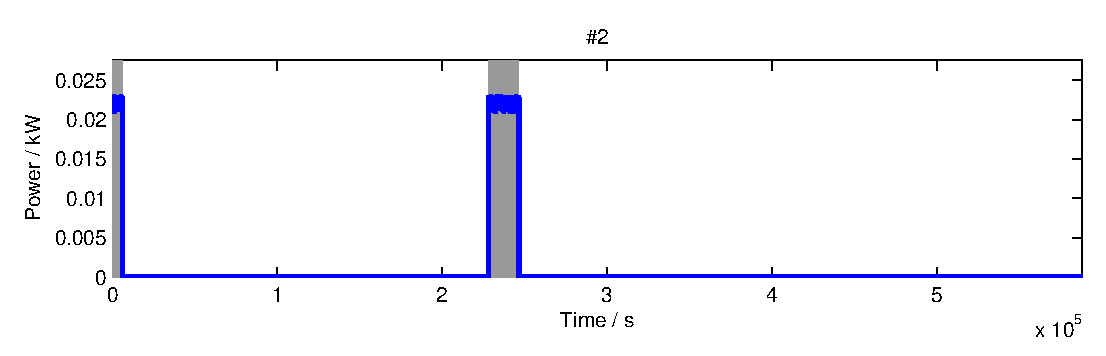
\includegraphics[width=\textwidth] {../../sw/pc/matlab/disagg-result/state-2.eps}
        \caption{\#2 Monitor}
    \end{subfigure}
    \\
    \begin{subfigure}[t]{0.8\textwidth}
        \centering
        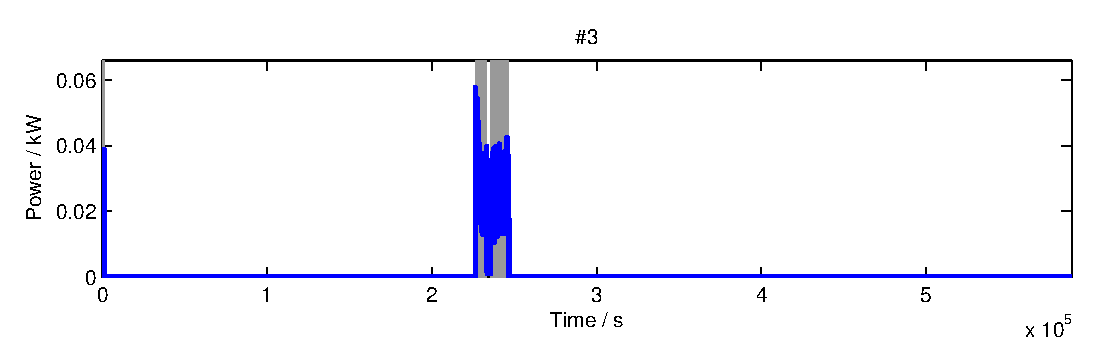
\includegraphics[width=\textwidth] {../../sw/pc/matlab/disagg-result/state-3.eps}
        \caption{\#3 Laptop}
    \end{subfigure}
    \\
    \begin{subfigure}[t]{0.8\textwidth}
        \centering
        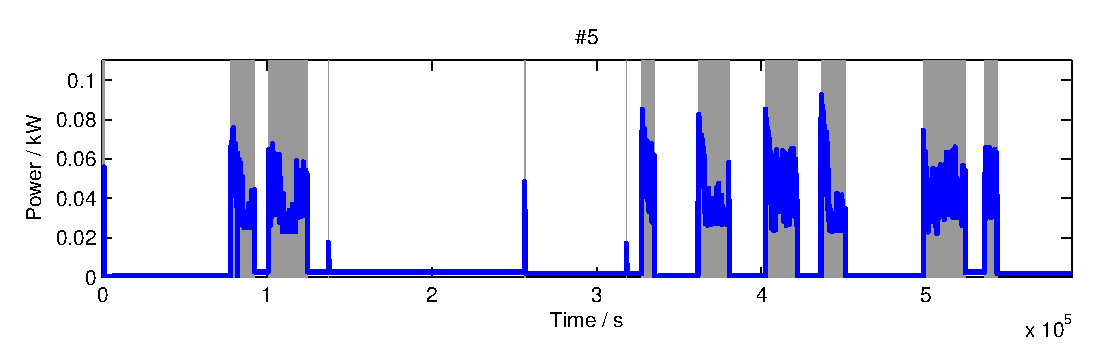
\includegraphics[width=\textwidth] {../../sw/pc/matlab/disagg-result/state-5.eps}
        \caption{\#5 Laptop}
    \end{subfigure}
    \caption{Appliance state reported vs. truth (\#1,2,3,5)}\label{fig:state-1-2-3-5}
\end{figure}

\begin{figure}[p]
    \centering
    \begin{subfigure}[t]{0.8\textwidth}
        \centering
        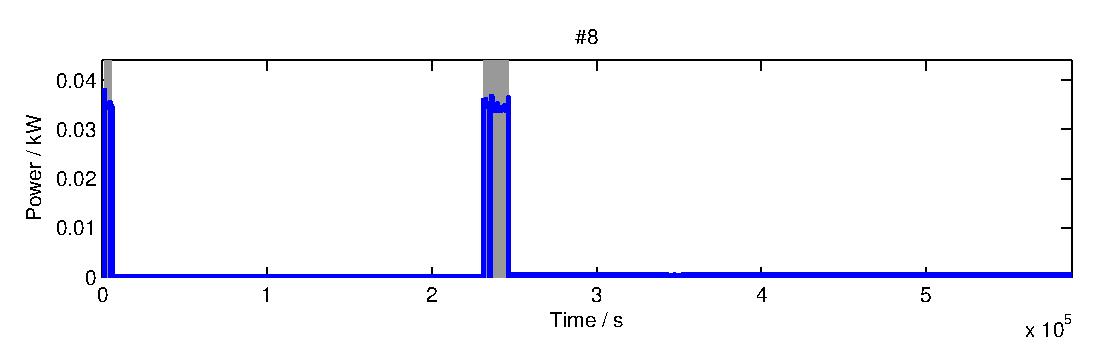
\includegraphics[width=\textwidth] {../../sw/pc/matlab/disagg-result/state-8.eps}
        \caption{\#8 Monitor}
    \end{subfigure} 
    \\
    \begin{subfigure}[t]{0.8\textwidth}
        \centering
        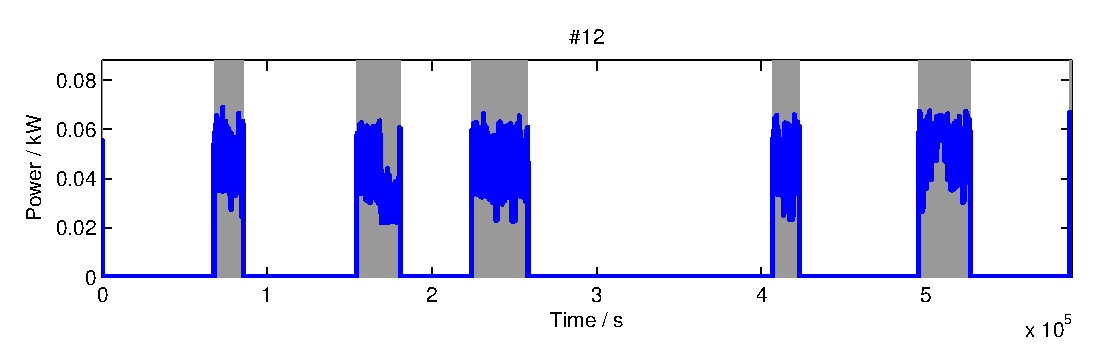
\includegraphics[width=\textwidth] {../../sw/pc/matlab/disagg-result/state-12.eps}
        \caption{\#12 Laptop}
    \end{subfigure}
    \\
    \begin{subfigure}[t]{0.8\textwidth}
        \centering
        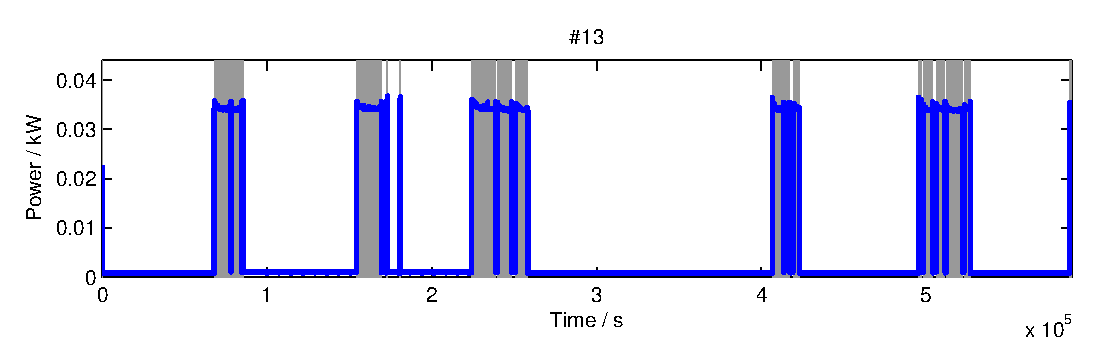
\includegraphics[width=\textwidth] {../../sw/pc/matlab/disagg-result/state-13.eps}
        \caption{\#13 Monitor}
    \end{subfigure}
    \\
    \begin{subfigure}[t]{0.8\textwidth}
        \centering
        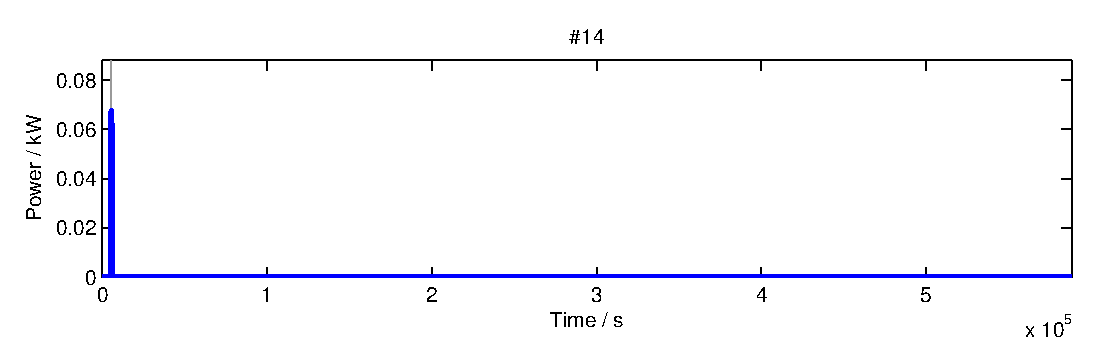
\includegraphics[width=\textwidth] {../../sw/pc/matlab/disagg-result/state-14.eps}
        \caption{\#14 Laptop}
    \end{subfigure}
    \caption{Appliance state reported vs. truth (\#8,12,13,14)}\label{fig:state-8-12-13-14}
\end{figure}

\begin{figure}[p]
    \centering
    \begin{subfigure}[t]{0.8\textwidth}
        \centering
        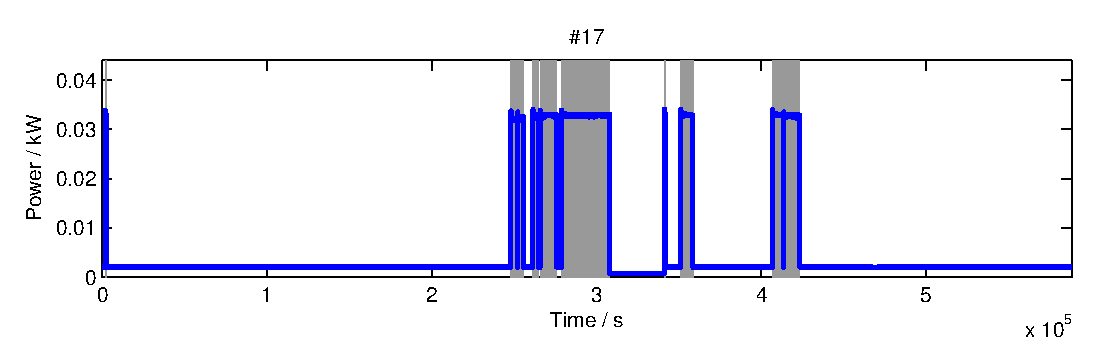
\includegraphics[width=\textwidth] {../../sw/pc/matlab/disagg-result/state-17.eps}
        \caption{\#17 Monitor}
    \end{subfigure} 
    \\
    \begin{subfigure}[t]{0.8\textwidth}
        \centering
        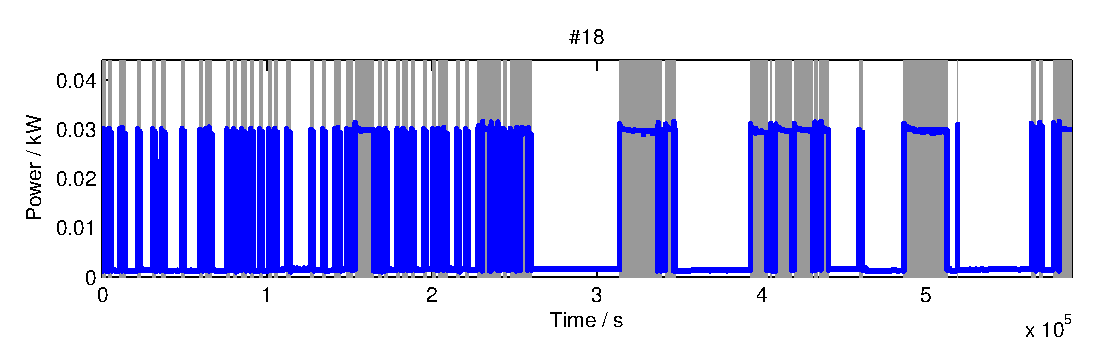
\includegraphics[width=\textwidth] {../../sw/pc/matlab/disagg-result/state-18.eps}
        \caption{\#18 Monitor}
    \end{subfigure}
    \\
    \begin{subfigure}[t]{0.8\textwidth}
        \centering
        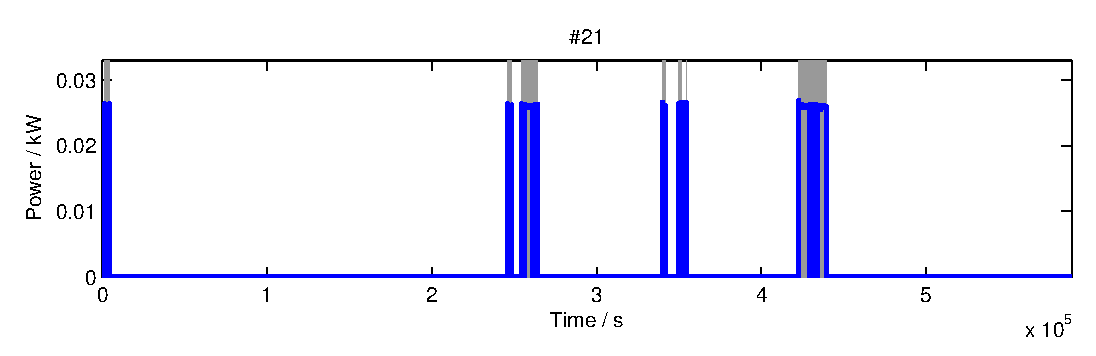
\includegraphics[width=\textwidth] {../../sw/pc/matlab/disagg-result/state-21.eps}
        \caption{\#21 Monitor}
    \end{subfigure}
    \caption{Appliance state reported vs. truth (\#17,18,21)}\label{fig:state-17-18-21}
\end{figure}


\subsection{Energy consumption of individual appliances}

Once we have reliable appliance power states and the step changes in the aggregated power, we can estimate the power traces of individual appliances, according to the algorithm discussed previously. 

Table \ref{tab:disagg} shows the energy consumption estimation of the appliances. For those appliances instrumented with ground truth power readings, we show both the true energy consumption over the 7-day period of the dataset, and the estimated energy consumption. For those appliances without ground truth power readings, only the estimation is shown. In the experiments, we found that appliance \#1 and \#2, which are two monitors, are working in complete synchrony. Theoretically, there is no way to distinguish the power consumption of them other than metering them separately. Hence, we regard them as a single combined appliance. 

The estimation error differs very much among different appliances. For most appliances, the error is less than 30\%. However, for monitors \#1+2, laptop \#3 and laptop \#5, the error is large. Generally, LCD monitors, which have stable on-state power, have more accurate results, while energy estimation for laptops are less accurate. This is because the power of an on-state laptop can vary as much as one third over time, due to different load, battery charging status, etc. Other causes of inaccuracy include lack of state changes. Some appliances are kept on or off for a long time, and there are only few state changes. In this case, the errors in the power step detection will keep accumulating. Monitors \#1+2 and laptop \#3 all fall in this case. They have just 3-5 state changes during the period of the dataset. 

Fig.\ref{fig:power-1-2-3-5-8}-\ref{fig:power-18-21} displays some snippets of estimated power vs ground truth for several appliances. 

\begin{table}
  \centering
  \begin{tabular}{lccccr}
  \hline
  ID & Power-on time (h) & Avg. power (W) & Energy (Wh) & Est. energy (Wh) & Error (\%) \\
  \hline
1+2& 6.85  & 47.9  & 327.9   &  163.0   &  -50.3 \\
3  & 5.31  & 29.9  & 158.9   &  233.8   &  +47.1 \\
5  & 37.87 & 38.6  & 1461.4  & 2279.1   & +56.0 \\
8  & 5.41  & 44.9  & 242.9   & 199.0    & -18.1 \\
12 & 35.76 & 36.9  & 1319.1  & 1639.1   & +24.3 \\
13 & 29.66 & 36.2  & 1072.1  & 1241.7   & +15.8 \\
14 & 0.21  & 63.1  & 13.4    & 9.60     & -28.3 \\
17 & 20.92 & 45.9  & 961.0   & 667.8    & -30.8 \\
18 & 60.68 & 31.1  & 1885.2  & 1718.3   & -8.9 \\
21 & 9.64  & 26.9  & 259.8   & 290.2    & +11.7 \\
  \hline
4 & 64730  & -  & -   & 537.7    & - \\
7 & 259984  & -  & -   & 17216    & - \\
9 & 521012  & -  & -   & 5697.8    & - \\
11 & 61032  & -  & -   & 829.0    & - \\
15 & 3852  & -  & -   & 47.9    & - \\
19 & 55160  & -  & -   & 324.7    & - \\
22 & 59216  & -  & -   & 640.6    & - \\
  \hline    
  \end{tabular}
  \caption{Energy consumption estimation of individual appliances}
  \label{tab:disagg}
\end{table}

\begin{figure}[p]
    \centering
    \begin{subfigure}[t]{\textwidth}
        \centering
        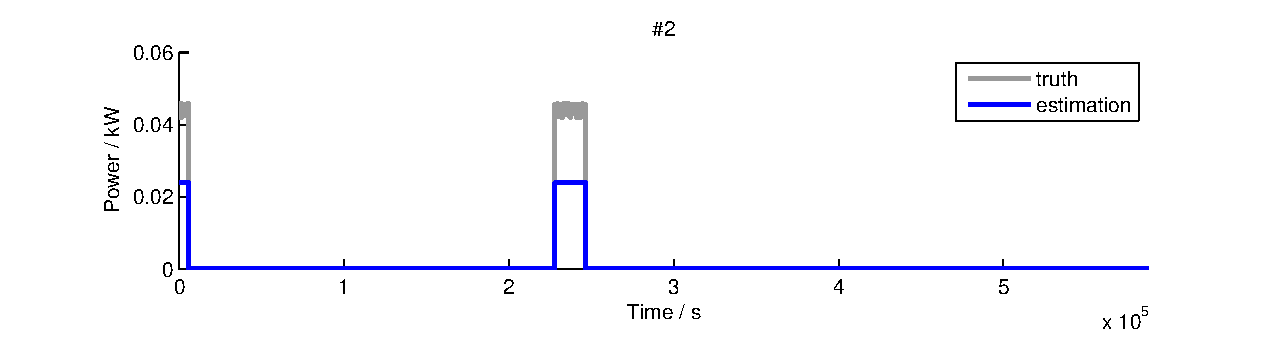
\includegraphics[width=\textwidth] {../../sw/pc/matlab/disagg-result/power-1-2.eps}
        \caption{\#1+2 Monitors}
    \end{subfigure} 
    \\
    \begin{subfigure}[t]{\textwidth}
        \centering
        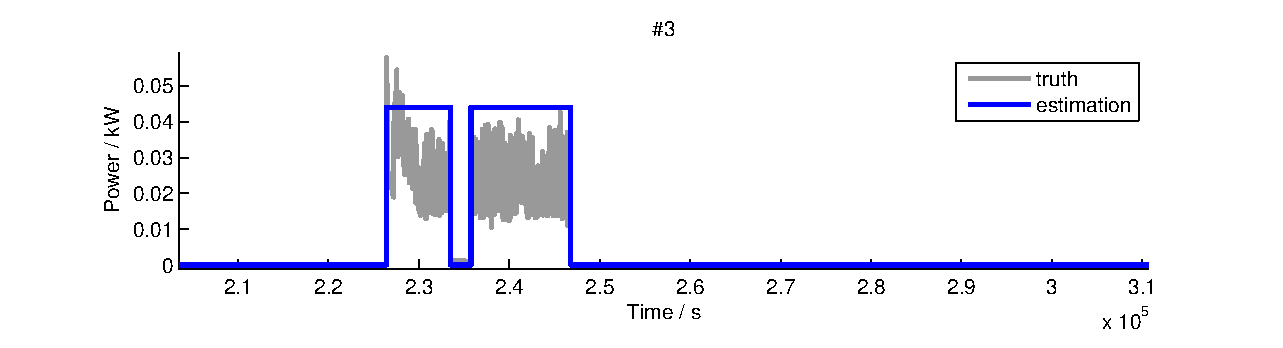
\includegraphics[width=\textwidth] {../../sw/pc/matlab/disagg-result/power-3.eps}
        \caption{\#3 Laptop}
    \end{subfigure}
    \\
    \begin{subfigure}[t]{\textwidth}
        \centering
        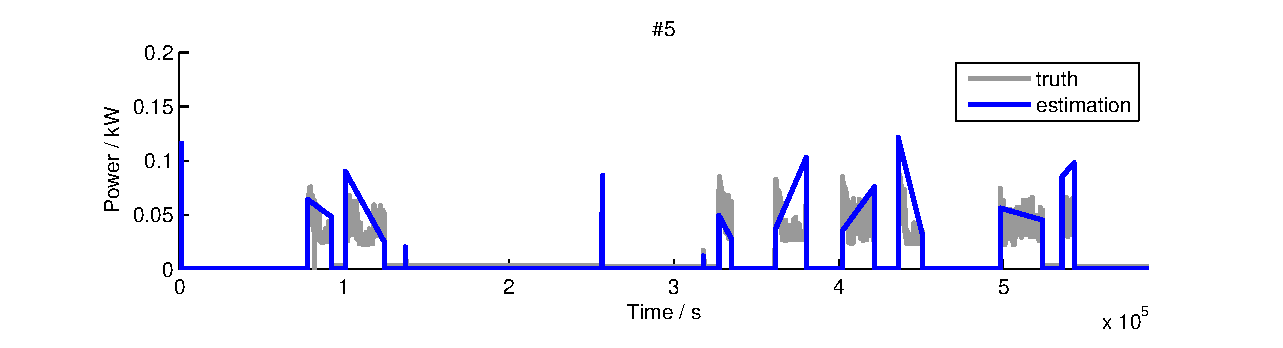
\includegraphics[width=\textwidth] {../../sw/pc/matlab/disagg-result/power-5.eps}
        \caption{\#5 Laptop}
    \end{subfigure}
    \\
    \begin{subfigure}[t]{\textwidth}
        \centering
        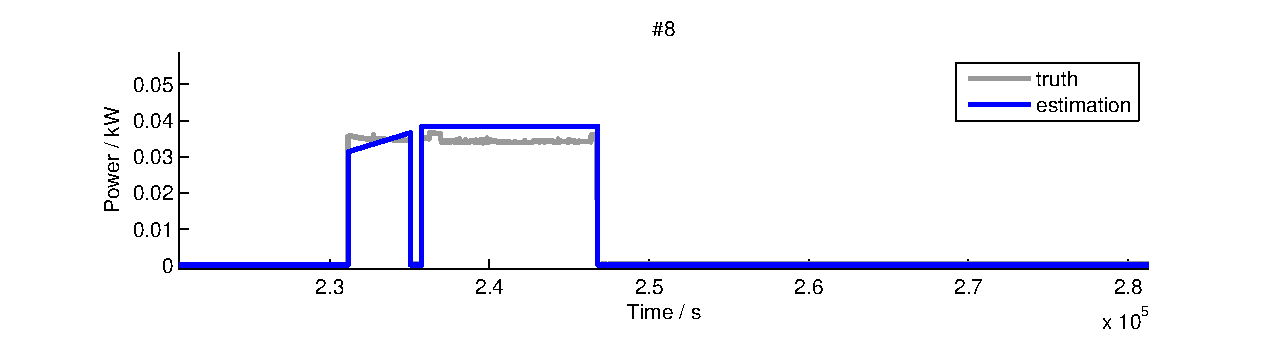
\includegraphics[width=\textwidth] {../../sw/pc/matlab/disagg-result/power-8.eps}
        \caption{\#8 Monitor}
    \end{subfigure}
    \caption{Appliance power consumption estimation vs. truth (\#1+2,3,5,8)}\label{fig:power-1-2-3-5-8}
\end{figure}

\begin{figure}[p]
    \centering
    \begin{subfigure}[t]{\textwidth}
        \centering
        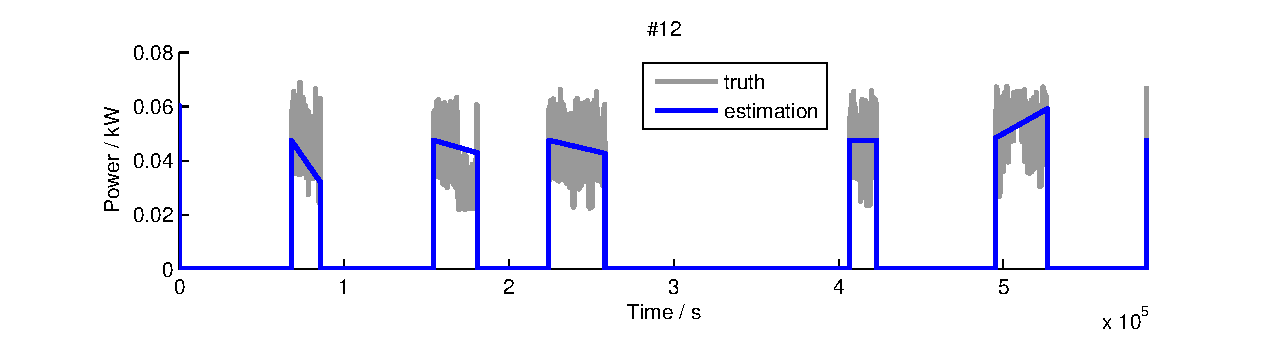
\includegraphics[width=\textwidth] {../../sw/pc/matlab/disagg-result/power-12.eps}
        \caption{\#12 Laptop}
    \end{subfigure} 
    \\
    \begin{subfigure}[t]{\textwidth}
        \centering
        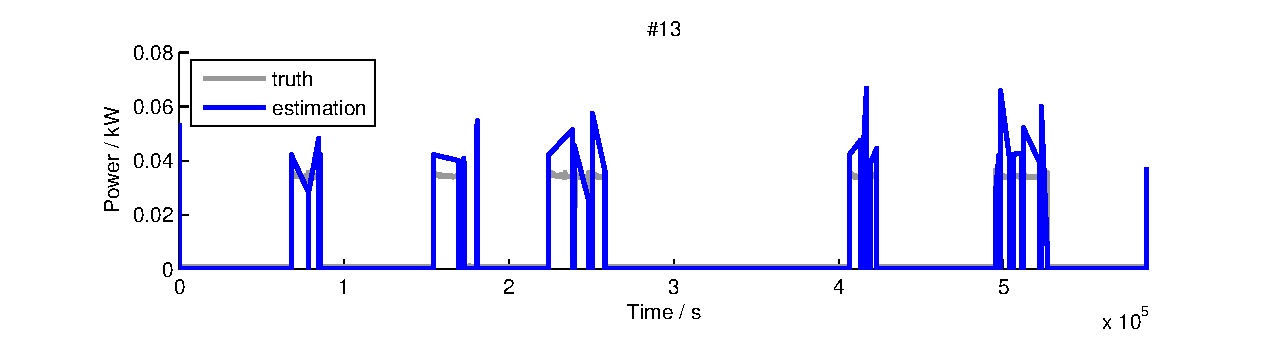
\includegraphics[width=\textwidth] {../../sw/pc/matlab/disagg-result/power-13.eps}
        \caption{\#13 Monitor}
    \end{subfigure}
    \\
    \begin{subfigure}[t]{\textwidth}
        \centering
        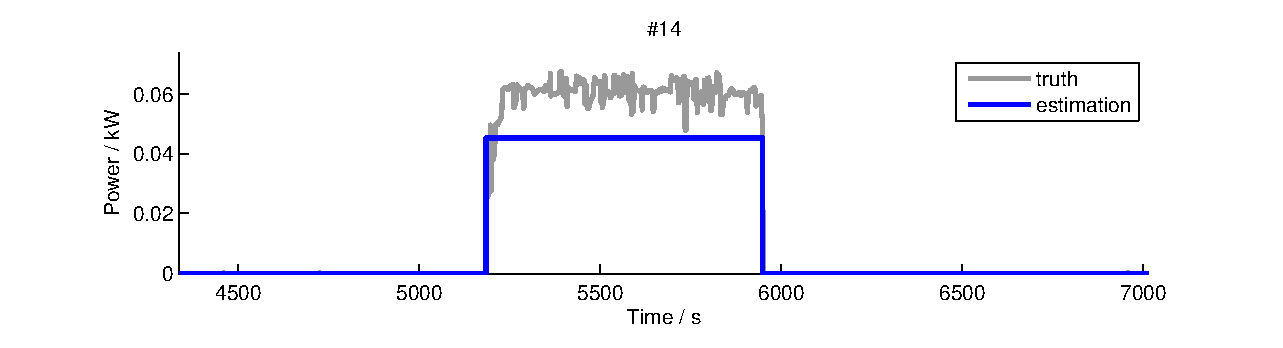
\includegraphics[width=\textwidth] {../../sw/pc/matlab/disagg-result/power-14.eps}
        \caption{\#14 Laptop}
    \end{subfigure}
    \\
    \begin{subfigure}[t]{\textwidth}
        \centering
        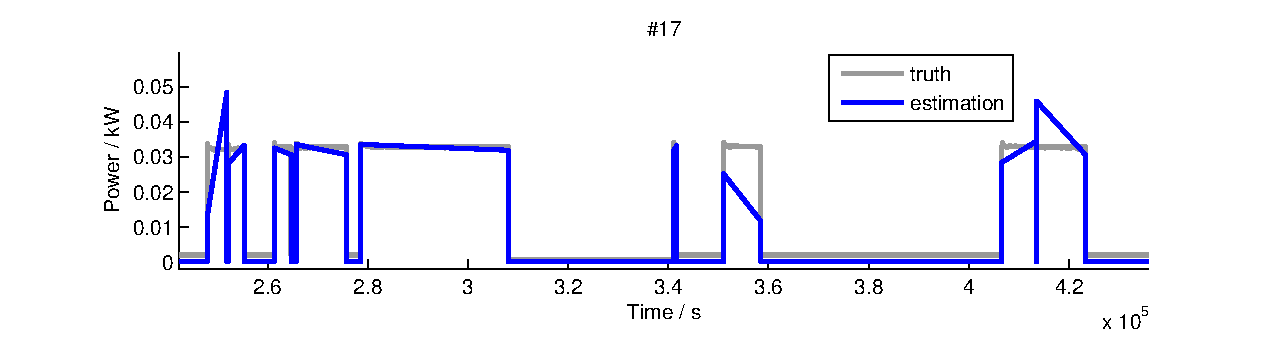
\includegraphics[width=\textwidth] {../../sw/pc/matlab/disagg-result/power-17.eps}
        \caption{\#17 Monitor}
    \end{subfigure}
    \caption{Appliance power consumption estimation vs. truth (\#12,13,14,17)}\label{fig:power-12-13-14-17}
\end{figure}

\begin{figure}[p]
    \centering
    \begin{subfigure}[t]{\textwidth}
        \centering
        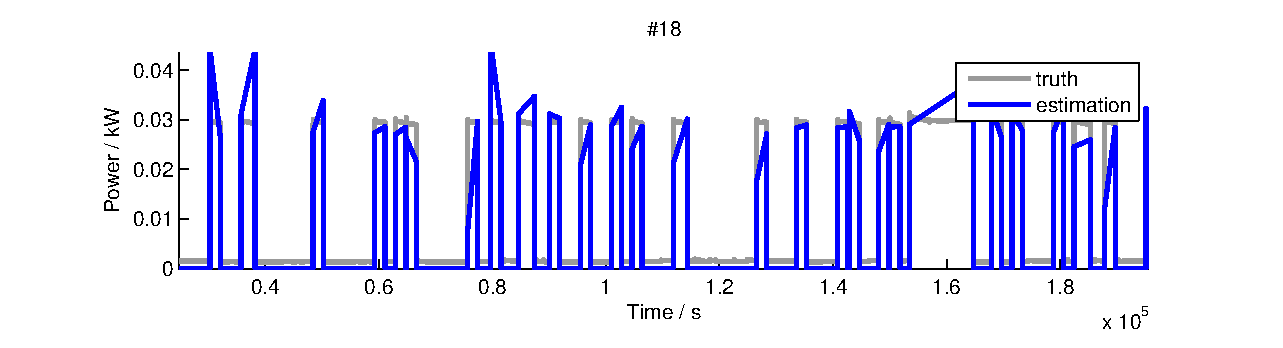
\includegraphics[width=\textwidth] {../../sw/pc/matlab/disagg-result/power-18.eps}
        \caption{\#18 Monitor}
    \end{subfigure} 
    \\
    \begin{subfigure}[t]{\textwidth}
        \centering
        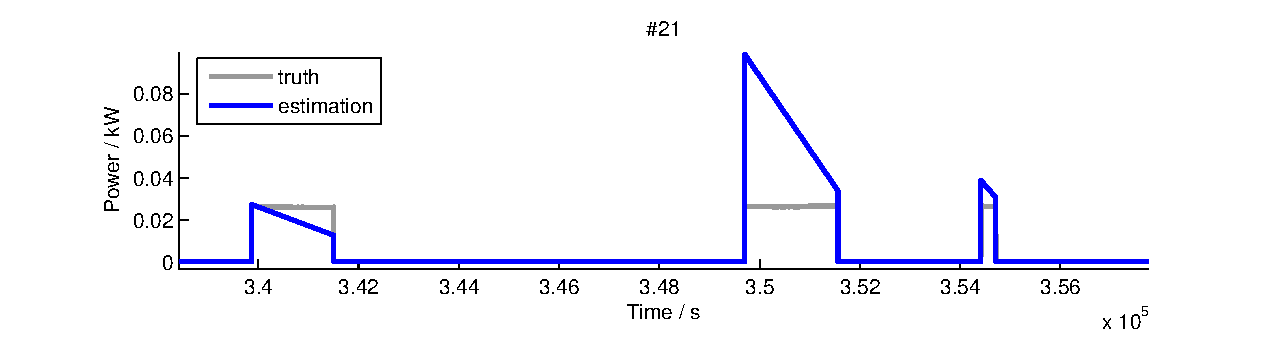
\includegraphics[width=\textwidth] {../../sw/pc/matlab/disagg-result/power-21.eps}
        \caption{\#21 Monitor}
    \end{subfigure}
    \caption{Appliance power consumption estimation vs. truth (\#18,21)}\label{fig:power-18-21}
\end{figure}
